\chapter{Background}
\label{chap:background}
\section{Multimodal sentiment analysis}
In traditional sentiment analysis, emotions are retrieved from textual information. Multimodal Sentiment Analysis (MSA) aims to generalize the standard text based sentiment analysis to videos where three communicative modalities are present: text, video, and acoustics. This focus on MSA is essential to understand human behavior, because human communication occur through both verbal and nonverbal cues. Therefore, when someone utter a sentence, the meaning of the utterance can drastically shift depending on the nonverbal behaviours. For example, the sentence ''The movie is sick'' is a ambiguous when perceived from a textual perspective because it can be considered both positive and negative. When you combine the utterance with a smile, the sentence will automatically become positive. When the speaker say the same sentence with a frown expression, it will be negatively loaded. A person speaking ''The movie is sick'' in a loudly voice will also be ambiguous. This means that visual features are powerful in describing something more effectively than words and can in particular be used to predict a sentiment with textual data. MSA systems may consist of a combination of two modalities such as text+video, text+speech, speech+video or all three. A system including two modalities is called a bimodal system whereas a system with all three modalities present is called a trimodal system. 

Modalities come in different forms including audio i.e. vocal words (e.g. utterances, tones, laughs), visual features (e.g. gestures, eye contact), and text (e.g. transcripts produced from audio data) or in the form of electroencephalography (EEG) signals \cite{MSA-review-3-9686504}. The text comprises of polar words where only a subset of the words contribute to the sentiment. It is also divided into word group or phrases, character N-Grams, and phoneme N-Grams in order to understand the context of the given text. Audio features are for example pitch, pauses, intonation, energy distribution over a sentence, and speed of an utterance. The visual indicators include smiles, frowns, gestures, posture, gazes, and eye contact. 

Figure \ref{fig:msa_process} illustrates the process of sentiment analysis by fusing several modalities. First, the unstructured data such as a video is taken as input and then pre-processed. In the pre-process phase, data is cleaned and filtered into audio, video, and textual data using various dimensionality reduction techniques. Then, features from audio, visual, and textual data is extracted using different feature methods.  
%
\begin{figure}[h]
  \centering
  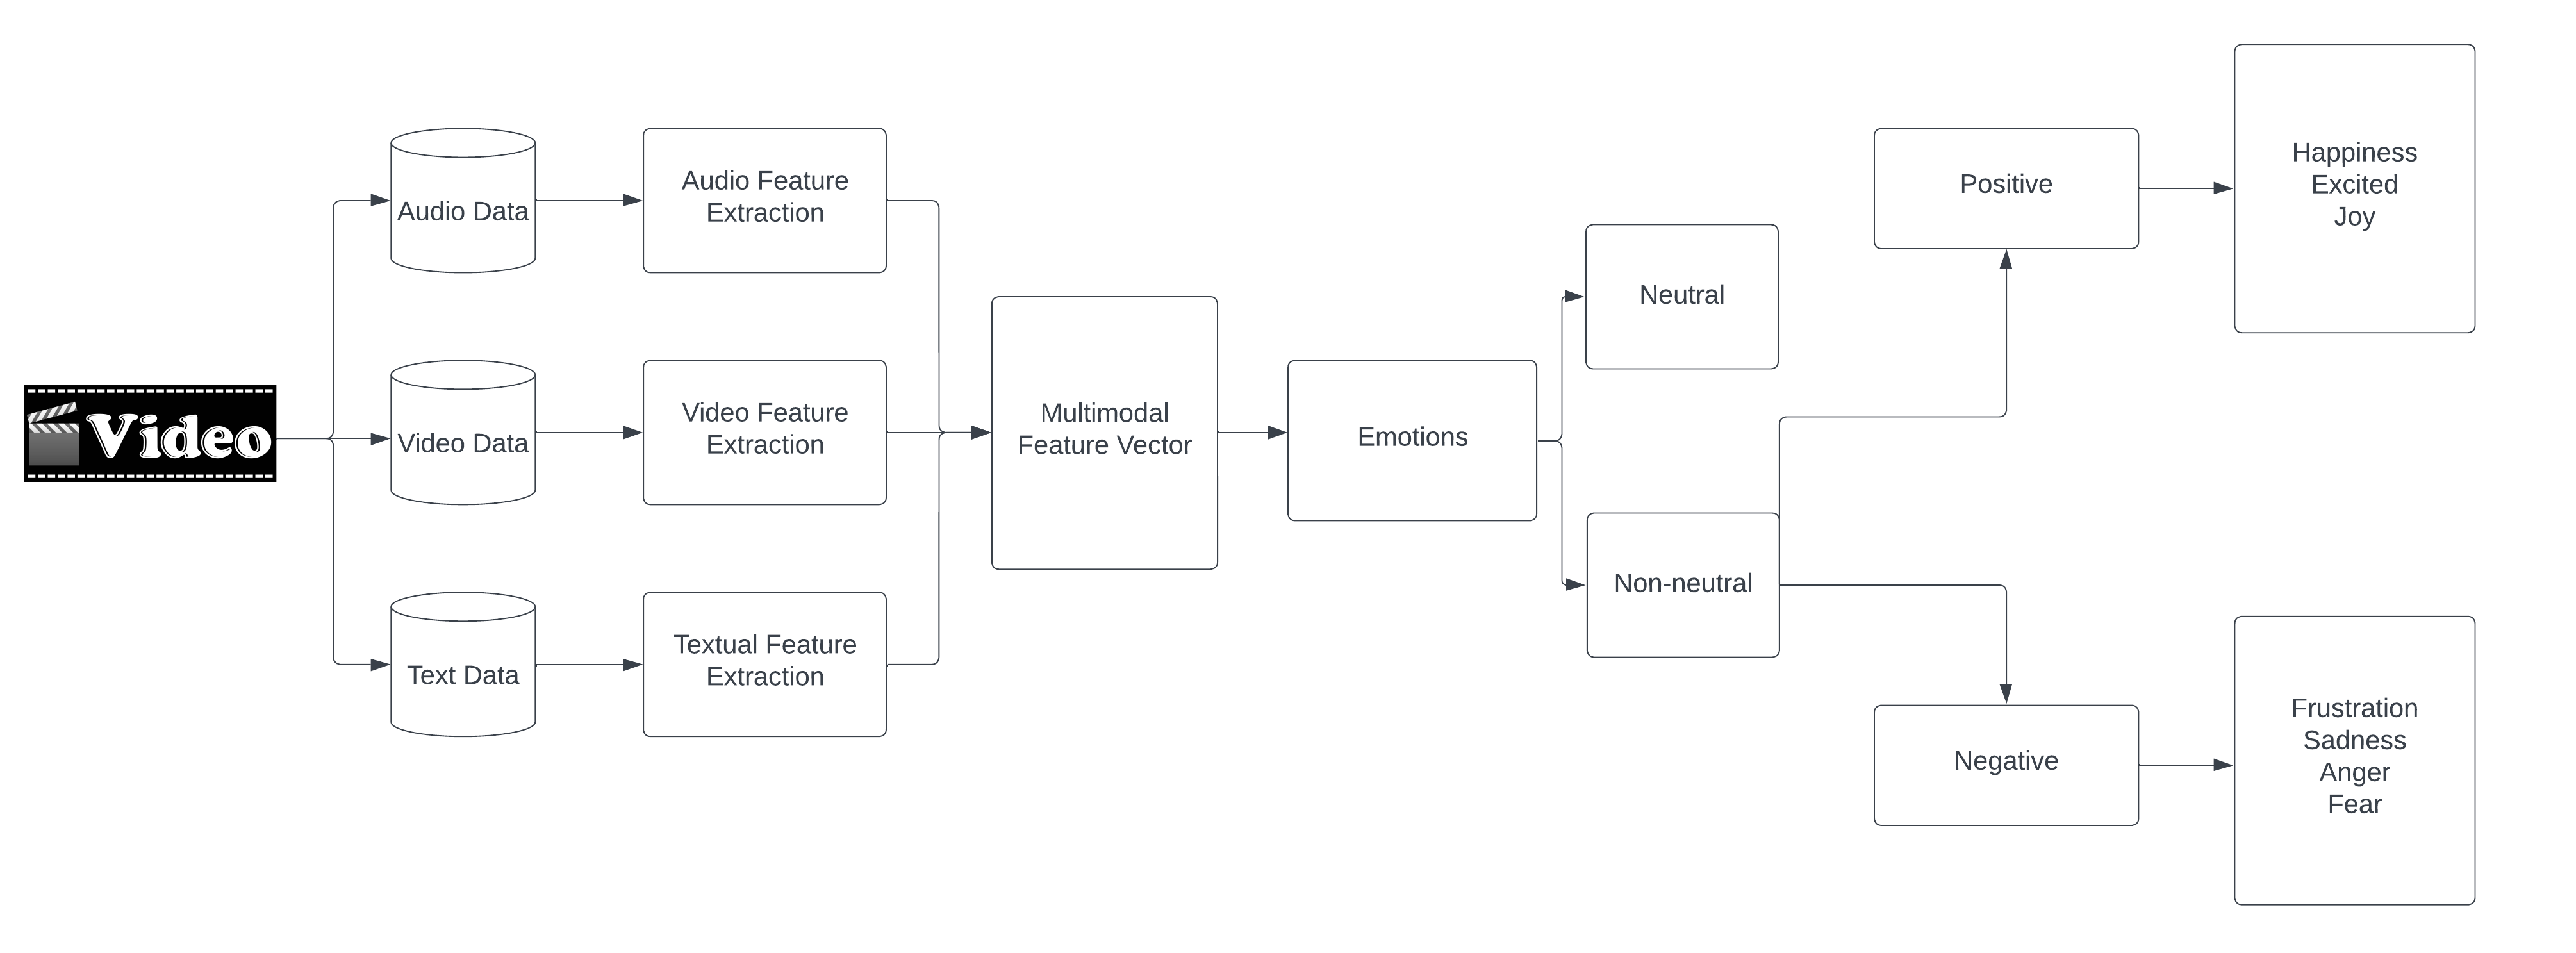
\includegraphics[width=1.0\textwidth]{figures/msa_process.png}
  \caption{MSA process.}
  \label{fig:msa_process}
\end{figure}
%
From the feature extraction phase, feature vectors are converted into decision feature vector for multiple modalities. Lastly, a classification algorithm categorizes the corresponding emotion based on the multimodal feature vector. Emotions can be classified as Neutral and Non-neutral. A neutral emotion denotes that no feelings are expressed to any circumstances. The non-neutral category consists of positive and negative emotions. Emotion classification can also be more fine-grained, where positive and negative emotions are divided into emotion classes (i.e. happy, excited, and joy for positive emotions and frustration, sadness, anger, and fear for negative emotions).

The most critical activity of MSA is fusion of multiple modalities. Fusion is the process of combining, filtering and extracting required features from the data accumulated from different modalities \cite{MSA-review-3-9686504}. Multimodal fusion is important because this data is used to classify the emotions. Currently, there are ten different multimodal fusion architectures:
%
\begin{itemize}
    \item \textbf{Early fusion-feature level fusion}: Feature level fusion, also called early fusion, merges the extracted features from visual, audio, and textual data into a high dimensional feature vector \cite{MSA_review2_GANDHI2023424}. Then, it is processed in the desired classification algorithm. 
    \item \textbf{Late fusion-decision level fusion}: In late fusion, the features of each modality is examined and classified independently before the results are fused together to form a final decision vector that predicts the emotion \cite{MSA-review-3-9686504}. 
    \item \textbf{Hybrid fusion}: Hybrid fusion utilizes both early and late fusion for emotion classification. When using hybrid fusion, the benefits of early and late fusion is exploited while their drawbacks are excluded at the same time.
    \item \textbf{Model-level fusion}: The characteristics of each modality is examined to find the correlation between them. The model is then developed in accordance with the research domain and given problem requirements \cite{MSA-review-3-9686504}. 
    \item \textbf{Tensor fusion}: With the use of a tensor fusion layer that explicitly imitates unimodal, bimodal, and trimodal interactions, this method creates a 3-fold Cartesian product. It reduces the quantity of training samples needed \cite{MSA_review2_GANDHI2023424}.
    \item \textbf{Hierarchical fusion}: As the name indicates, this fusion process fuses the features in an hierarchical order. Here, the model starts to merge the modalities two in two first, and then all three modalities \cite{MSA_review2_GANDHI2023424}.
    \item \textbf{Bimodal fusion}: In bimodal fusion, two different modality pairs are used as input to deal with the information imbalance between modalities. The two components are trained concurrently so they can duel in a simulated combat \cite{MSA_review2_GANDHI2023424}.
    \item \textbf{Attention mechanism-based fusion}: Attention mechanism-based fusion aims to incorporate multi-level contextual feature extraction. To do this, the model uses attention-based inter-modality fusion at utterance level since each modality contributes differently to sentiment and emotion classification. Contextual attentive unimodal features are joined two by two to create bimodal features. These two sets of features are then combined to form trimodal feature vectors \cite{MSA_review2_GANDHI2023424}.
    \item \textbf{Quantum based fusion}: In this method, quantum inference is used to capture the interactions within each utterance (i.e. correlations between different modalities). Additionally, quantum measurement is used to build a strong-weak influence model to find the interactions between consecutive utterances (i.e. how one speaker is influenced by another). Quantum based fusion also utilizes decision-level or early fusion techniques \cite{MSA-review-3-9686504}. 
    \item \textbf{Word level fusion}: This method investigates the interplay between different modalities in order to establish a superior sentiment tendency. Transformer is used to learn joint representations for utterances and to translate across different modalities \cite{MSA_review2_GANDHI2023424}. 
\end{itemize}

\section{The use of video interviews in e-recruitment}
As young people are staying in education longer than ever, they become very attractive in the labour market. Everyone desires to get their dream job, and selecting the best candidates that fit well with the job-description is essential to meet the employer's expectations. Like every other aspect with business today, the hiring process depends on speed and accuracy \cite{hiring-process-Sołek-BorowskaWilczewska+2018+25+33}. The job market has become more competitive due to an increasing number of highly relevant candidates competes against a decreasing pool of jobs. Additionally, the selection process is relatively short meaning that the hiring managers have to precisely choose the most suited candidates. The integration of both software and hardware in the HR sector is an emerging trend to keep up with the speed of recruitment and selection. Technologies such as Big Data, Internet of Things, Deep Learning, Machine Learning, and Artificial Intelligence have impact on the HR industry \cite{robotic-process-nawaz2019robotic}. Hiring managers rely on automated systems to help them assess candidates at a fast pace. Some automated systems include  applicant tracking systems \cite{ATS2015} where the system can view your resume and collect keywords to see how well you fit with the job description, surveys \cite{ONEILL2013162} in order to assess your behaviours at the workplace, and automated video interviews \cite{Chen2017_video_interview} in order for the corporation to get to know your communication skills.   \\

A well conducted recruitment and selection process is important for any organizations as it empower in-depth and objective verification of candidates \cite{hiring-process-Sołek-BorowskaWilczewska+2018+25+33}. How different organizations conduct the hiring process varies and there is not one way to do so. However, several industries such as Consulting, Finance, Computer Science, and Engineering are utilizing automated video interviews and is a central part of their e-recruitment process. Automated interviews, also called asynchronous video interviews (AVIs), on-demand interview, web-based interview, pre-recorded interview, etc., is a new form of video interviews. Instead of real-time communication between the interviewer and the interviewee, the candidates communicate one way asynchronous by recording their answers to interview questions for representatives from the organization to evaluate at a later time \cite{video-interview1-LUKACIK2022100789}. AVIs have several advantages. It is faster, cheaper and requires less employment time than live interviews \cite{video_interview2-brenner2016asynchronous}. This enables organizations assessing a broader pool of possible candidates. The AVI interview setting has increased reliability and validity since it incorporates principles from structured interviews \cite{video-interview1-LUKACIK2022100789}. Additionally, AVI recordings are easy to store and share without information loss. This allows multiple evaluators to assess each candidate, enabling the recruiters to form a collective decision in the selection.   \\

One crucial aspect with AVIs is their design \cite{video-interview1-LUKACIK2022100789}. AVI design indicate the structure of the interview that is created by a combination of different features. The design make each AVI unique, and design choices will impact the outcome applicant behavior, and organizations and hiring manager reactions. Therefore, corporations need to carefully choose their set of AVI features with the purpose of the associated AVI. Table \ref{tab:AVI-design-features} shows AVI design features that is taken into consideration when creating AVIs. The response formatting features is the core of the AVI method. The duration a question is presented, the time to prepare a question answer, and the ability to re-record a response will affect the interviewee and these features need to be adjusted depending on the outcome desired by each company. For example, having a short question timer, a short response preparation time, and a limited re-recording possibility results that candidates have to do their best at the first try. In this way they may express more emotions through their vocal responses but also from their behaviors. However, this feature setting increases the applicants' anxiety and decreases the candidate fairness perception. If these features are moved to the other side of the spectrum, allowing people to complete the interview at their own pace, the previous consequences are mitigated. But, the downside with this feature setting is that applicants are now able to produce well formulated responses where it can be challenging to monitor the emotions expressed. Another important feature consideration is the evaluation features. The AVI can be evaluated by human evaluators or automatically analyzed by an AI-system. Utilizing only AI-systems interrelated with increased AVI invitation refusal because automated systems can be worse in assessing job performance information than human evaluators. Nevertheless, automated assessment can reduce bias such as negative impact against particular groups (e.g. age, gender, ethnicity) and visual appearance (e.g. attractiveness). In practise, a combination of both human evaluators and AI-systems are used for evaluation of candidates. In this way, the evaluators can assess each candidate's personality rapidly before making a decision. Table \ref{tab:AVI-applicant-choices} lists the choices applicants have associated with an AVI. Some of these choices may affect the performance of each candidate. For example, completing an interview after a long work day may lead to poorer communication skills because the applicants is not as mentally sharp as in the beginning of the day. The choices can also affect the evaluators' perception of the interviewee. At one hand, the automated evaluator will not perceive anyone differently as long as the connection speed and image clarity is above the specified requirements. At the other hand, human evaluator are influenced by applicant location, background content, and physical appearance. Additionally, a video setting with appropriate lighting, high image clarity and stability is rated more positively. 
%
\begin{table}[h]
    \caption{AVI design features.}
    \centering
    \resizebox{\columnwidth}{!}{%
    \begin{tabular}{l p{9.4cm}}
     \toprule
     \multicolumn{2}{c}{\textbf{Structure and formatting features}} \\ \\
     Question timers	& The duration a question is presented for the applicant. The question can be showed within a limited time, or be presented until the user performs an action (i.e. clicking a button to acknowledge they have understood the question). \\
     \midrule
     \multicolumn{2}{c}{\textbf{Media features}} \\ \\ 
     Video introductions & The use of videos, audio clips, photos, music, etc. in the AVI. This may include introduction videos to the organization or interview or videos of the workplace. \\ \\ 
     Video recorded questions & The interview questions is prerecorded by an ''interviewer'' in comparison to read the questions on paper. \\ \\
     Media quality & The production quality in AVIs. This include image resolution, aesthetics, acting, sound quality, etc. \\
     \midrule 
     \multicolumn{2}{c}{\textbf{Response formatting features}} \\ \\ 
     Response preparation time & The time each candidate has to prepare a question answer. Questions can be showed right before the recording happens, or it can be a part of the interview invitation. \\ \\ 
     Re-recording responses & The ability to re-record a response after previous attempts. Attempts for re-recording can be limited or candidates can have endless tries. \\ \\ 
     Interrupted interview completion & The time allowed for a candidate to pursue the interview. This can include unlimited time to complete the interview without timing out, or the ability for the candidates to leave and resume the interview at a later time. \\ \\ 
     Length of allowed response & The total length allowed for the candidate's response to an interview question. The duration can be specified or left indefinite until the applicant performs an action. \\ \\ 
     Ability to review response & The ability to review the recorded response before moving on with the next question or to re-record the same question. \\ \\ 
     Video recording preview & A live recording preview window. \\ 
     \midrule
     \multicolumn{2}{c}{\textbf{Evaluation features}} \\ \\ 
     Human evaluator(s) & Multiple people can evaluate the interview to establish a collective decision. \\ \\ 
     Automated assessment & Interview are automatically analyzed using machine learning/deep learning techniques. These automated models are able to assess candidates' personality. \\ 
     \bottomrule
    \end{tabular}
    }
    \label{tab:AVI-design-features}
\end{table}
%
\begin{table}[h]
    \caption{Choices done by applicants associated with an AVI.}
    \centering
    \resizebox{\columnwidth}{!}{%
    \begin{tabular}{l p{9.4cm}}
    \toprule
    \multicolumn{2}{c}{\textbf{Time and location choices}} \\ \\
    Location of interview & The location the candidate chooses to perform the interview. This can be at home, at the office, etc. \\ \\ 
    Background content & Visible objects in the background such as furniture, pictures, and artwork that can provide additional information about the applicant. \\ \\ 
    Time of day & The time of the day the candidate performs the interview (i.e. daytime or nighttime). \\ \\ 
    Physical appearance/Attire & Applicant's chosen aesthetics when recording responses. \\
    \midrule
    \multicolumn{2}{c}{\textbf{Technology choices}} \\ \\ 
    Connection speed & The connection speed may affect the video outcome in terms of clear audio and good image resolution. \\ \\ 
    Image clarity/Stability & The image clarity is impacted by the way candidates choose to perform the interview. Applicants may use different devices including laptops, tablets, and phones which affect the image stability. \\ 
    \bottomrule
    \end{tabular}
    }
    \label{tab:AVI-applicant-choices}
\end{table}

\begin{comment}
Everyone desires to get their dream job. Either it is as a developer, teacher, accountant, etc., the common aspect to these fields is that to acquire the positions, the candidates have to go through a challenging hiring process. As the job market is becoming more competitive and the hiring process to fill job positions is relatively short, recruiters rely on automatic systems to help them extract candidates that fit well with the job description. Some of the automated systems include applicant tracking systems \cite{ATS2015}, surveys \cite{ONEILL2013162}, and automated video interviews \cite{Chen2017_video_interview}. The latter is an essential stage of the recruitment process because this is your chance to showcase your communication skills as well as nonverbal cues such as facial expression, body language, and paralanguage so the recruiters can assess your personality. The candidate's personality is among the top three factors companies look for in employment and in some cases personality is ranked above both education and appearance \cite{important_personality}. \\ 
\end{comment}

\section{Big-five model}
Researchers have for several decades applied methods to develop a personality taxonomy that describes personality traits \cite{personality_goldberg_1990}. One of the most known psychology theory is the big five personality traits. This model is the result of the work conducted by researchers including Fiske \cite{fiske1949consistency}, Norman \cite{norman19672800}, Smith \cite{smith1967usefulness}, Goldberg \cite{goldberg1981language}, and McCrae and Costa \cite{mccrae1987validation}. The five basic dimensions of personality are - Openness, Conscientiousness, Extraversion, Agreeableness, and Neuroticism. 
%
\begin{figure}[h]
  \centering
  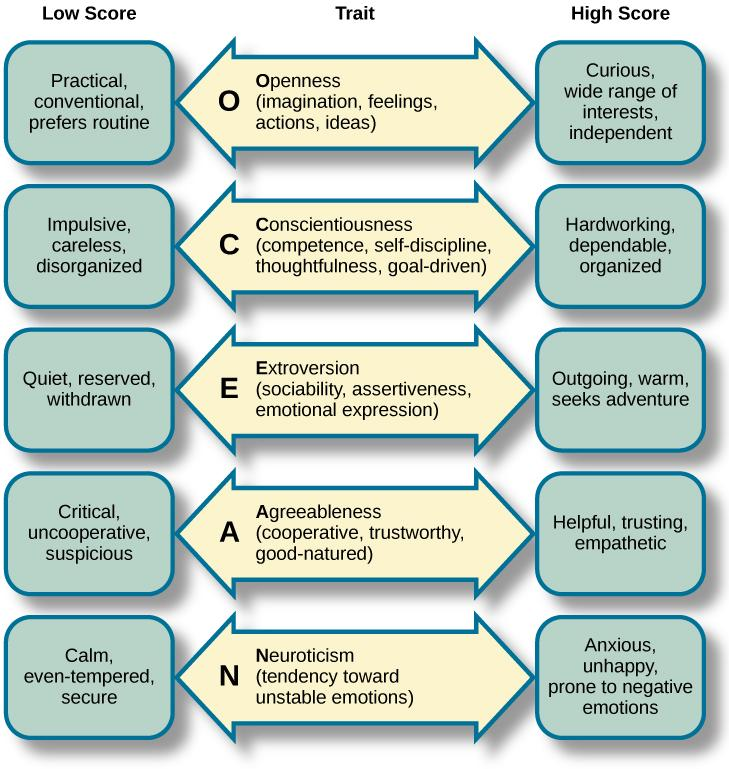
\includegraphics[width=0.5\textwidth]{figures/big-5-personality.jpeg}
  \caption{The big five personality traits. [17]}
  \label{fig:big5}
\end{figure}
%
Since the model's dimensions are broad, it covers all personality traits aspects. As shown in Figure \ref{fig:big5} \cite{big5-image}, the big five  represent the personality traits as a spectrum where it identifies what is considered a low and high score for each trait. Based on job performance, according to \cite{best_trait}, the best personality trait is conscientiousness. A person with a high score in conscientiousness has knowledge, good leadership skills, and is more desired to learn.

\section{COGMEN}
The Contextualized Graph neural network based Multimodal Emotion recognition (COGMEN) model focuses on exploiting contextual information, inter-speaker and intra-speaker relations in a conversation setting \cite{COGMEN_joshi-etal-2022-cogmen}. This means that the framework addresses key concepts to capture emotions in a conversation: It leverages the overall context in the dialogue referred to as the global information. Also, it utilizes the local information stored in the conversations to monitor the emotion expressed by each speaker and create relations between the syllables. In essence, COGMEN is made up of four different modules that are responsible of predicting the emotion of an input utterance. The first module is called Context Extractor. Each input utterance consist of concatenated features from visual, acoustic, and textual modalities. The Context Extractor utilizes a transformer encoder in capturing the global information from each input utterance. With newly established context features, these attributes are fed into the second module, Graph Formation. This unit forms the features to a graph where each statement act as a node of the graph and they are connected using directed relations. Here, there exist two type of relations: relation between utterances by the same speaker (intra-relations) and relations between utterances from different speakers (inter-relations). Next, the third model is Relational GCN and GraphTransformer. The RGCN uses the graph as input to capture intra-speaker and inter-speaker dependencies. Then, the GraphTransformer supplements the RGCN by extracting rich representations from the node features by considering nodes that are connected via edges. Last, the fourth module is the Emotion Classifier. Based on features extracted in the previous step, a linear classifier is utilized to predict the emotion for each utterance.




